\section{Development Evidence: Sealed Test of the Full Head}
\label{supp:development}
Before the shift gate existed, the full head (the 108-column forecaster without the gate) was tested on a sealed cohort of 120 new kernels from the generator families, 84 of them stochastic, with 22 registered contrasts. Table~\ref{tab:forecast} reports its scores. Against B2 matched it lowers IBS from 0.05473 to 0.04599 (15.97\%) and LL from 0.62718 to 0.56308 (10.22\%), with simultaneous lower bounds $+0.00275$ and $+0.02981$, and all 22 contrasts, including two privileged rows with access to the true MDP, have positive simultaneous bounds. The raw OEH-B law alone is poorly calibrated (IBS 0.09783, LL 0.91068), so the gain comes from the fitted combination. Fig.~\ref{fig:threshold} breaks the IBS down by budget threshold: both forecasters are calibrated in the large, and the full head's advantage is sharper discrimination, concentrated at $x5$--$x50$ for BC and IQL and at $x10$--$x20$ for CFQI. By learner, the descriptive intervals exclude zero for CFQI and IQL and cross zero for BC (90.71\% censored); by family, the gain is large for Garnet ($-30.0\%$ IBS), moderate for forward-layered MDPs and absent for the 18 bottleneck MDPs. These results concern a component of the final method and were obtained on a cohort that later served for development.

\begin{table}[t]
\centering
\caption{Sealed forecast scores on 84 new stochastic MDPs (lower is better). Gain: relative improvement of the full head; LB: simultaneous one-sided 95\% lower bound on the absolute improvement (22 contrasts).}
\label{tab:forecast}
\small
\setlength{\tabcolsep}{3pt}
\resizebox{\columnwidth}{!}{%
\begin{tabular}{@{}lcccc@{}}
\toprule
Forecast inputs & IBS & LL & Gain (IBS/LL) & LB (IBS/LL)\\
\midrule
\multicolumn{5}{@{}l}{\emph{Matched head, pilot only (Tier 1)}}\\
B2 matched & .05473 & .6272 & 16.0/10.2\% & .0027/.030\\
B2 + ERI adapt. & .05667 & .6330 & 18.9/11.0\% & .0041/.034\\
B2 + BWD adapt. & .05395 & .6212 & 14.8/9.4\% & .0023/.025\\
\midrule
\multicolumn{5}{@{}l}{\emph{Other heads, pilot only (Tier 1)}}\\
B2 generic (AFT) & .06399 & .7824 & 28.1/28.0\% & .0104/.146\\
Train frequency & .10953 & .9428 & 58.0/40.3\% & .0482/.314\\
\midrule
\multicolumn{5}{@{}l}{\emph{Matched head, privileged (Tier 2)}}\\
B2 + oracle EH & .05471 & .6266 & 15.9/10.1\% & .0024/.026\\
B2 + TQ/SACo & .05221 & .6142 & 11.9/8.3\% & .0010/.023\\
\midrule
Raw OEH-B (no head) & .09783 & .9107 & \multicolumn{2}{c}{reported, not gated}\\
Full head (108 columns) & \textbf{.04599} & \textbf{.5631} & --- & ---\\
\bottomrule
\end{tabular}}
\end{table}

\begin{figure}[t]
\centering
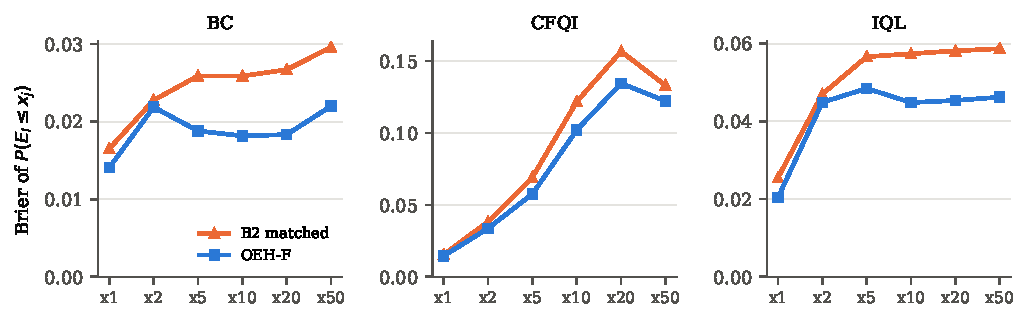
\includegraphics[width=\columnwidth]{figures/fig_threshold_brier.pdf}
\caption{Brier score of the cumulative forecast $P(E_l\le x_j)$ at each budget threshold on the 84 stochastic MDPs (420 rows per learner). The integrated Brier score of Table~\ref{tab:forecast} averages these six values. Mean forecast and observed attainment rates agree closely for both methods (calibration table in the released artifacts); the difference is in discrimination.}
\label{fig:threshold}
\end{figure}
